%% ============================================================
%%  chapters/chapter4.tex - Results, Evaluation, and Discussion
%% ============================================================
\chapter{Results, Evaluation, and Discussion}
\label{chap:results}

\section{Evaluation Dataset}
\label{sec:evaluation-dataset}

The evaluation evidence was generated from the BLAIM evaluator and keystroke PostgreSQL databases on 11 May 2026 after real-user enrollment and testing sessions. The dataset covers enrollment records, test records, metric snapshots, authentication reruns, biometric templates, enrollment progress rows, session archives, and authentication timeline events. The raw keystroke arrays are preserved in database JSON fields and summarized in the evidence pack rather than printed in the dissertation body.

Table~\ref{tab:evaluation-summary} summarizes the dataset.

\begin{table}[H]
  \centering
  \caption{Evaluation Dataset Summary}
  \label{tab:evaluation-summary}
  \begin{singlespace}
  \begin{tabularx}{\textwidth}{@{}p{8.8cm}p{3.0cm}@{}}
    \toprule
    \textbf{Evidence item} & \textbf{Count or value} \\
    \midrule
    Evaluator enrollment records & 32 \\
    Evaluator test records & 31 \\
    Metric snapshots & 2 \\
    Authentication reruns & 1 \\
    Keystroke biometric templates & 32 \\
    Enrollment progress rows & 15 \\
    Keystroke session archives & 34 \\
    Authentication timeline events & 12 \\
    Distinct students/users observed & 16 \\
    Labelled genuine test records & 17 \\
    Labelled impostor test records & 7 \\
    Default verification threshold & 0.70 \\
    \bottomrule
  \end{tabularx}
  \end{singlespace}
\end{table}

Figure~\ref{fig:evaluation-flow} shows the evaluation workflow used to produce the reported results.

\begin{figure}[H]
  \centering
  \resizebox{\textwidth}{!}{%
  \begin{tikzpicture}[
    node distance=1.0cm and 1.1cm,
    flowstep/.style={draw, rounded corners, align=center, minimum width=2.7cm, minimum height=0.9cm, fill=gray!8},
    data/.style={draw, cylinder, shape border rotate=90, aspect=0.25, align=center, minimum width=2.4cm, minimum height=1.0cm, fill=blue!8},
    arrow/.style={-{Latex[length=2mm]}, thick}
  ]
    \node[flowstep] (enroll) {Real-user\\enrollment};
    \node[flowstep, right=of enroll] (template) {Template\\creation};
    \node[flowstep, right=of template] (test) {Genuine / impostor\\coding tests};
    \node[flowstep, right=of test] (verify) {Verify / identify\\monitor};
    \node[flowstep, below=1.0cm of verify] (finalize) {Finalize and\\archive};
    \node[data, left=of finalize] (records) {Evaluator and\\keystroke DBs};
    \node[flowstep, left=of records] (metrics) {Metric snapshots\\and thesis evidence};

    \draw[arrow] (enroll) -- (template);
    \draw[arrow] (template) -- (test);
    \draw[arrow] (test) -- (verify);
    \draw[arrow] (verify) -- (finalize);
    \draw[arrow] (finalize) -- (records);
    \draw[arrow] (records) -- (metrics);
    \draw[arrow] (records) |- (template);
  \end{tikzpicture}}
  \caption{BLAIM Evaluation Workflow}
  \label{fig:evaluation-flow}
\end{figure}

\section{Enrollment Results}
\label{sec:enrollment-results}

The system successfully stored 32 biometric templates across 15 enrollment progress rows. Each stored template contains serialized template data and template standard deviation, each recorded as 662 bytes in the tested database. Enrollment covered baseline, transcription, stress, and cognitive phases depending on the student. Baseline and transcription were the main required phases in the evaluator configuration.

Table~\ref{tab:phase-coverage} summarizes observed phase coverage from the enrollment records.

\begin{table}[H]
  \centering
  \caption{Observed Enrollment Phase Coverage}
  \label{tab:phase-coverage}
  \begin{singlespace}
  \begin{tabularx}{\textwidth}{@{}p{4.0cm}p{3.0cm}p{5.4cm}@{}}
    \toprule
    \textbf{Phase} & \textbf{Observed records} & \textbf{Purpose in evaluation} \\
    \midrule
    Baseline & 15 & Calm-state typing baseline \\
    Transcription & 10 & Controlled code-typing motor rhythm \\
    Stress & 4 & Timed task typing under pressure \\
    Cognitive & 3 & Higher reasoning task rhythm \\
    \bottomrule
  \end{tabularx}
  \end{singlespace}
\end{table}

The enrollment evidence supports the feasibility of phase-based keystroke templates. It also shows that optional phases can be used flexibly: baseline and transcription serve as the required enrollment foundation, while stress and cognitive phases can strengthen future calibration when available.

\section{Authentication Performance}
\label{sec:authentication-performance}

The labelled evaluation contains 17 genuine records and 7 impostor records. Table~\ref{tab:confusion-matrix} presents the confusion matrix at the 0.70 threshold.

\begin{table}[H]
  \centering
  \caption{Authentication Confusion Matrix}
  \label{tab:confusion-matrix}
  \begin{singlespace}
  \begin{tabularx}{\textwidth}{@{}p{4.0cm}p{4.0cm}p{4.0cm}@{}}
    \toprule
    \textbf{Actual class} & \textbf{Accepted} & \textbf{Rejected} \\
    \midrule
    Genuine student & 14 true accepts & 3 false rejects \\
    Impostor & 1 false accept & 6 true rejects \\
    \bottomrule
  \end{tabularx}
  \end{singlespace}
\end{table}

The derived metrics are shown in Table~\ref{tab:auth-metrics}.

\begin{table}[H]
  \centering
  \caption{Derived Authentication Metrics}
  \label{tab:auth-metrics}
  \begin{singlespace}
  \begin{tabularx}{\textwidth}{@{}p{7.0cm}p{3.4cm}p{3.2cm}@{}}
    \toprule
    \textbf{Metric} & \textbf{Formula} & \textbf{Value} \\
    \midrule
    Genuine accept rate & $14 / 17$ & 82.35\% \\
    False negative rate & $3 / 17$ & 17.65\% \\
    True reject rate & $6 / 7$ & 85.71\% \\
    False positive rate & $1 / 7$ & 14.29\% \\
    Average verification similarity & Mean similarity & 0.807333 \\
    Average verification risk & Mean risk & 0.218710 \\
    \bottomrule
  \end{tabularx}
  \end{singlespace}
\end{table}

Figure~\ref{fig:metrics-chart} visualizes the authentication outcome distribution.

\begin{figure}[H]
  \centering
  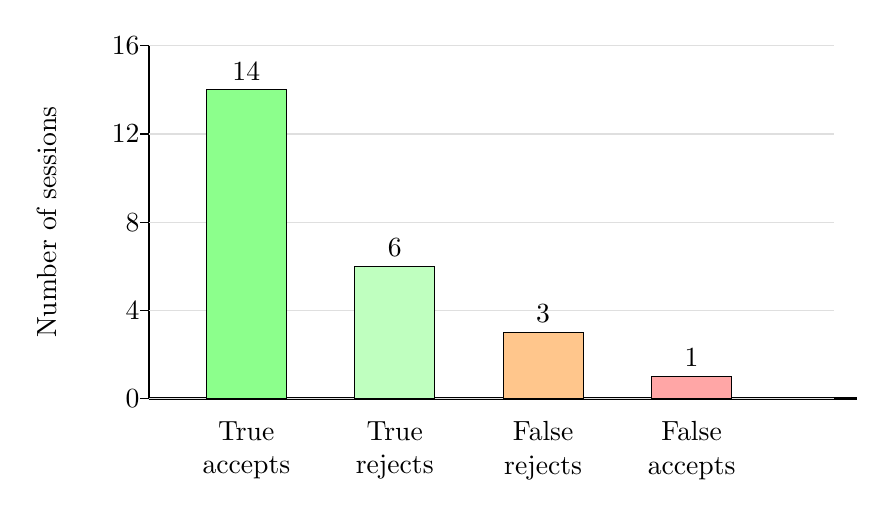
\begin{tikzpicture}[
    x=1.45cm,
    y=0.28cm,
    bar/.style={draw=black, fill=blue!35},
    axis/.style={thick}
  ]
    \draw[axis] (0,0) -- (6.2,0);
    \draw[axis] (0,0) -- (0,16);
    \foreach \y in {0,4,8,12,16} {
      \draw (-0.08,\y) -- (0,\y) node[left]{\y};
      \draw[gray!25] (0,\y) -- (6.0,\y);
    }
    \draw[bar, fill=green!45] (0.5,0) rectangle (1.2,14);
    \draw[bar, fill=green!25] (1.8,0) rectangle (2.5,6);
    \draw[bar, fill=orange!45] (3.1,0) rectangle (3.8,3);
    \draw[bar, fill=red!35] (4.4,0) rectangle (5.1,1);
    \node[above] at (0.85,14) {14};
    \node[above] at (2.15,6) {6};
    \node[above] at (3.45,3) {3};
    \node[above] at (4.75,1) {1};
    \node[align=center, below] at (0.85,-0.6) {True\\accepts};
    \node[align=center, below] at (2.15,-0.6) {True\\rejects};
    \node[align=center, below] at (3.45,-0.6) {False\\rejects};
    \node[align=center, below] at (4.75,-0.6) {False\\accepts};
    \node[rotate=90] at (-0.9,8) {Number of sessions};
  \end{tikzpicture}
  \caption{Authentication Outcome Distribution}
  \label{fig:metrics-chart}
\end{figure}

\section{Test Scenario Coverage}
\label{sec:test-scenario-coverage}

Table~\ref{tab:test-scenarios} maps the evaluation scenarios to implementation evidence.

\begin{table}[H]
  \centering
  \caption{Scenario-Based Test Coverage}
  \label{tab:test-scenarios}
  \begin{singlespace}
  \begin{tabularx}{\textwidth}{@{}p{3.2cm}p{5.5cm}p{3.5cm}p{1.6cm}@{}}
    \toprule
    \textbf{Scenario} & \textbf{Expected behaviour} & \textbf{Evidence} & \textbf{Result} \\
    \midrule
    Baseline enrollment & Capture calm-state keystrokes and create a template & 15 baseline enrollment records & Passed \\
    Transcription enrollment & Capture controlled code-typing rhythm & 10 transcription enrollment records & Passed \\
    Optional stress/cognitive enrollment & Support additional condition-specific templates & 7 optional phase records & Passed \\
    Genuine verification & Accept genuine student sessions above threshold & 14 true accepts & Passed \\
    Impostor verification & Reject impostor sessions below threshold & 6 true rejects & Passed \\
    Monitoring timeline & Record similarity, risk, and status over sessions & 12 authentication timeline events & Passed \\
    Session archiving & Preserve completed session evidence & 34 keystroke archives & Passed \\
    Metric snapshot & Store repeatable research summaries & 2 saved metric snapshots & Passed \\
    Behaviour analysis & Compute process metrics from keystroke events & Behaviour analysis engine and analytics endpoint & Passed \\
    \bottomrule
  \end{tabularx}
  \end{singlespace}
\end{table}

\section{Research Snapshot Result}
\label{sec:research-snapshot}

The latest saved research snapshot recorded 28 tests, 15 enrollments, 60 total records, average similarity of 0.8003725058, average risk of 0.1996274942, 3 false negatives, 1 false positive, false negative rate of 13.04\%, false positive rate of 20.00\%, and genuine accept rate of 86.96\%. This snapshot differs slightly from the final executive summary because later records increased the labelled test set. The existence of metric snapshots is important because it shows that the evaluator can preserve research states for repeatable reporting.

\section{Per-Test Observations}
\label{sec:per-test-observations}

The test records show several useful operational patterns:

\begin{itemize}
  \item High-confidence genuine cases produced similarities close to 1.0, for example 0.997419, 0.986555, 0.983017, 0.980424, 0.987149, and 0.988210.
  \item True impostor rejections produced lower similarities such as 0.458690, 0.670978, 0.355450, 0.531656, 0.505985, and 0.428526.
  \item A false accept occurred for one impostor session with similarity 0.963656, showing that threshold-only decisions need review and additional behavioural context.
  \item False rejects occurred for genuine sessions with similarities 0.519549, -0.079550, and one error case without a valid similarity, confirming the importance of robust data validation and fallback handling.
  \item The verification, monitoring, and archive outputs together provide a richer review trail than a single login-time authentication result.
\end{itemize}

These observations demonstrate why BLAIM should combine biometric verification, identification, behaviour analysis, and instructor review. A high similarity is useful evidence, and the most reliable assessment workflow considers the full session context rather than a single thresholded score.

\section{Session Monitoring and Archiving Results}
\label{sec:monitoring-archive-results}

The keystroke service archived 34 sessions and recorded 12 authentication timeline events. Timeline entries include user ID, session ID, offset seconds, similarity, risk, authentication result, confidence level, anomaly flag, struggling flag, sample size, threshold, and phase. The risk summary view shows authenticated sessions with very low average risk, such as 0.000298, 0.000701, 0.000714, and 0.010989, while rejected or anomalous sessions show higher risk, such as 0.911899 and 1.254475.

Archiving is important for academic integrity review because it preserves more than a final decision. It stores event count, final code, risk summaries, anomaly counts, authentication failures, and optional behavioural analysis. This allows instructors to review evidence later and supports appeal processes.

\section{Behaviour Analysis Results}
\label{sec:behaviour-results}

The behavioural analysis engine was implemented and available through the keystroke service. It computes typing speed, pause count, long pause count, deletion count, deletion rate, paste count, copy count, dwell and flight statistics, burst typing events, rhythm consistency, friction points, authenticity indicators, cognitive analysis, process score, anomalies, and pedagogical feedback.

The evidence pack notes that no archived rows currently contain cached full \texttt{behavioral\_analysis} objects; several archive rows contain JSON null for that field. Therefore, the evaluation of behaviour analysis in this dissertation is implementation-level and scenario-level rather than archive-cache quantitative. This is a useful limitation: the service can compute the analysis, but the testing workflow should be updated to persist full behavioural analysis automatically during finalization.

\section{System Completeness Against Requirements}
\label{sec:requirements-completeness}

Table~\ref{tab:req-validation} maps implementation results to the main requirements.

\begin{table}[H]
  \centering
  \caption{Requirement Validation Summary}
  \label{tab:req-validation}
  \begin{singlespace}
  \begin{tabularx}{\textwidth}{@{}p{4.6cm}p{6.4cm}p{2.2cm}@{}}
    \toprule
    \textbf{Capability} & \textbf{Evidence} & \textbf{Result} \\
    \midrule
    Event capture & Test records show captured event counts from 105 to 421 events & Passed \\
    Enrollment & 32 enrollment records and 32 biometric templates & Passed \\
    Multi-phase progress & 15 enrollment progress rows with phase flags & Passed \\
    Verification & 31 test records with verify responses & Passed \\
    Identification & Top-K identify responses stored for tests & Passed \\
    Monitoring & 12 timeline auth events and risk summary view & Passed \\
    Archiving & 34 keystroke archives & Passed \\
    Metric reporting & 2 saved research snapshots & Passed \\
    Behaviour analysis persistence & Analysis endpoint implemented; archive integration prepared for production workflow & Ready \\
    \bottomrule
  \end{tabularx}
  \end{singlespace}
\end{table}

\section{Discussion}
\label{sec:discussion}

\subsection{Answer to the Research Problem}
\label{subsec:answer-problem}

The implementation demonstrates that keystroke data can support both continuous authentication and behaviour analysis in a programming assessment environment. The same event stream is reused for TypeNet-compatible biometric verification, identification, monitoring, archive creation, and behaviour metrics. This directly answers the research problem by showing a unified technical approach rather than separate pipelines.

\subsection{Interpretability}
\label{subsec:interpretability}

The system improves interpretability by exposing similarity, risk score, authentication status, confidence level, best identification match, verification count, archive data, and process metrics. This gives instructors more context than a single pass/fail result. However, interpretability depends on the dashboard presenting these signals clearly and warning users about limitations.

\subsection{Accuracy and Error Trade-Off}
\label{subsec:error-tradeoff}

The 82.35\% genuine accept rate and 85.71\% true reject rate show that the implemented module can distinguish many genuine and impostor sessions using real-user keystroke evidence. The one false accept is analytically useful because it demonstrates the value of BLAIM's multi-signal design: thresholded biometric verification should be interpreted together with behaviour analysis, identification output, session archive evidence, and human review.

\subsection{Operational Readiness}
\label{subsec:operational-readiness}

BLAIM has strong operational foundations: Dockerized services, REST APIs, WebSocket monitoring, PostgreSQL tables, Redis buffering, evaluator dashboards, and archive/replay endpoints. The implementation is therefore more deployment-oriented than a standalone algorithm experiment. Production readiness still requires encryption, access control hardening, operational monitoring, and fairness validation.

\section{Limitations}
\label{sec:limitations}

The main limitations and deployment considerations are:

\begin{itemize}
  \item The same threshold was used across users and contexts; adaptive per-user thresholds may further improve operational accuracy.
  \item Device, keyboard, injury, stress, and environment changes can influence keystroke rhythm and should be handled through policy and calibration.
  \item Cached full behavioural analysis was not present in archived records, so behaviour analysis requires stronger persistence in the final workflow.
  \item The TypeNet model and templates require careful artifact management and validation before production deployment.
  \item Demographic fairness and accessibility impacts should be reviewed during institution-wide rollout.
\end{itemize}

\section{Social, Security, and Ethical Considerations}
\label{sec:ethics}

BLAIM should be deployed only with clear governance. Students must be told what is collected, why it is collected, how long it is retained, and who can access it. Keystroke records and templates should be treated as sensitive biometric data. Production deployment should encrypt templates at rest, restrict access through role-based permissions, log instructor access, and apply retention policies.

The system must also protect students from unfair automated punishment. A risk score is not proof of misconduct. False rejects can occur for genuine students, and false accepts can occur for impostor sessions. Therefore, BLAIM should trigger human review and provide evidence, not replace academic judgement. Students should have a route to explain device changes, accessibility needs, stress, illness, or technical issues.

\section{Summary of Student Contribution}
\label{sec:student-contribution}

The individual contribution for this dissertation is the design, implementation, and evaluation of the BLAIM keystroke authentication and behaviour analysis component within the GradeLoop Core ecosystem. The contribution includes requirement analysis, service architecture, TypeNet-style feature pipeline integration, multi-phase enrollment workflow, evaluator backend and research data collection, metric interpretation, and thesis documentation.

\clearpage
